% currently only working for 16:9 slides
% using 4:3 will cause the footer to be misaligned
\documentclass[aspectratio=169]{beamer}


\usepackage{xcolor}
\usepackage{amsmath}
\usepackage{tcolorbox}
\usepackage{listings}
\usepackage{url}

% dbs or uni
\usetheme{uni}



\title{Federated Learning With Individualized Differential Privacy By Client Sampling}
\subtitle{}
\author{Ole Borchardt}
\urldef{\mail}\path|ob14dupe@studserv.uni-leipzig.de|
\institute{Leipzig University}
\date{21.05.2024}


\usepackage[backend=bibtex, style=authoryear-comp]{biblatex}
\addbibresource{references.bib}
\newcommand{\tinycite}[1]{\tiny{\citeauthor{#1}, \citetitle{#1}, \citeyear{#1}}} 
\newcommand{\normalcite}[1]{\citeauthor{#1}, \citetitle{#1}, \citeyear{#1}} 
\addtobeamertemplate{footnote}{}{\vspace{4ex}}

\usepackage{tikz}
\usepackage{ocgx2}
\usetikzlibrary{positioning}

\begin{document}
\setbeamertemplate{caption}{\raggedright\insertcaption\par}
  
\maketitlepage

\begin{frame}
\tableofcontents[hideallsubsections]
\end{frame}

\section{Introduction}

\begin{frame}{Motivation and Goal}
    \begin{itemize}
        \item Federated Learning (FL) a mechanism to train models on collaboratively among multiple clients
        \begin{itemize}
            \item keeps the training data at the clients
            \item only model updates are shared
            \item allows to train models collaboratively and to adapt the model to individual clients
            \item information may still be leaked due to exchanged data and the influence on the final model
        \end{itemize} 
    \end{itemize}
\end{frame}

\begin{frame}{Motivation and Goal}
    \begin{itemize}
        \item Differential Privacy (DP) can limit the leakage of information
        \begin{itemize}
            \item provides a defense mechanism against various attacks on privacy (e.g. membership inference attacks)
            \item Performance-privacy trade-off
        \end{itemize}
        \item<2-> Individualized DP can minimize performance cost
        \begin{itemize}
            \item individual users may have individual privacy needs
            \item idea is to utilize the individual privacy budgets to full capacity instead of applying one budget to all clients
        \end{itemize}
    \end{itemize}
\end{frame}

\subsection{Basics of Differential Privacy}

\begin{frame}{Differential Privacy}
    \begin{itemize}
        \item Goal is to limit the influence of individuals on a query result
    \end{itemize}
\end{frame}

\begin{frame}
    \begin{block}{$(\epsilon, \delta)$-Differential Privacy (DP)}
        A \textit{randomized mechanism} $\mathcal{M}: \mathcal{D} \rightarrow \mathcal{R}$ with domain $\mathcal{D}$ and range $\mathcal{R}$ satisfies $(\textcolor{red}{\epsilon}, \textcolor{blue}{\delta})$-differential privacy if for any two adjacent inputs $d$, $d' \in \mathcal{D}$ and for any subset of outputs $S \subseteq \mathcal{R}$ it holds that $$\Pr[\mathcal{M}(d) \in S] \leq e^{\textcolor{red}{\epsilon}} \Pr[\mathcal{M}(d') \in S] + \textcolor{blue}{\delta}$$
    \end{block}
    \begin{itemize}
        \item<2-> $\textcolor{red}{\epsilon}$ is called Privacy Budget
        \item<2-> $\textcolor{blue}{\delta}$ is the probability that privacy is broken (preferably $\textcolor{blue}{\delta} < 1 / |d|$)
        \item<3-> typically adjacent inputs refer to two datasets that differ in one record
        \item<3-> favorable characteristics under composition and for releasing DP-results
    \end{itemize}
\end{frame}

\begin{frame}{Realization of DP-Mechanisms}
    \begin{itemize}
        \item there are a few mechanisms that are proven to fulfill DP when choosing appropriate parameters
        \begin{itemize}
            \item Laplace-Mechanism, Exponential Mechanism, Randomized Response, \textbf{Gaussian Mechanism}
            \item typically add noise to the results with a variance that depends on parameters 
        \end{itemize}
        \item<2-> noise also depends on \textbf{sensitivity} $s$
        \begin{itemize}
            \item maximum difference in the result between adjacent datasets ($s = 1$ in a count query, ...)
            \item for vectors the $\ell_2$ norm is used as a measure of sensitivity
        \end{itemize}
        \item<3-> additional theorems exist for the \textbf{composition} of DP-Queries 
    \end{itemize}
\end{frame}

% \begin{frame}{Gaussian Mechanism}
%     \begin{itemize}
%         \item adds Gaussian Noise with $\mu = 0$ and $\sigma^2 \geq \frac{2s^2\ln(1.25 / \delta)}{\epsilon}$ to a Query Result \parencite{dwork:2014}
%         \item $s$ is called \textit{sensitivity}
%         \begin{itemize}
%             \item maximum difference between two records
%             \item $s = 1$ in a count query, ...
%             \item captures the influence a single data point may have on the query result
%         \end{itemize}
%     \end{itemize}
% \end{frame}

% \begin{frame}{Querying data multiple times}
%     \begin{itemize}
%         \item the same data is queried $k$ times 
%         \item Composition Theorem\parencite{dwork:2014}
%         \begin{itemize}
%             \item $\mathcal{M}_{[k]}(x) = (\mathcal{M}_1(x), ..., \mathcal{M}_k(x))$, $\mathcal{M}_1, ..., \mathcal{M}_k$ are $(\epsilon_i, \delta_i)$-differentally private
%             \item then $\mathcal{M}_{[k]}$ is $(\sum\epsilon_i, \sum\epsilon_i)$-differentially private
%             \item very broad upper bound of $\epsilon$ (grows linearly with $k$)
%         \end{itemize}
%         \item Strong Composition Theorem grows with $\sqrt{k}$
%         \item even better bounds for ML with the Moments Accountant
%     \end{itemize}
% \end{frame}

% \begin{frame}{Releasing differentially private data}
%     \begin{itemize}
%         \item result was obtained via an $(\epsilon, \delta)$-differentially private mechanism
%         \item any post-processing will still be $(\epsilon, \delta)$-differentially private \parencite{dwork:2014}
%     \end{itemize}
% \end{frame}

\subsection{Differential Privacy in Machine Learning}

\begin{frame}
    \begin{figure}[tb]
      \centering
      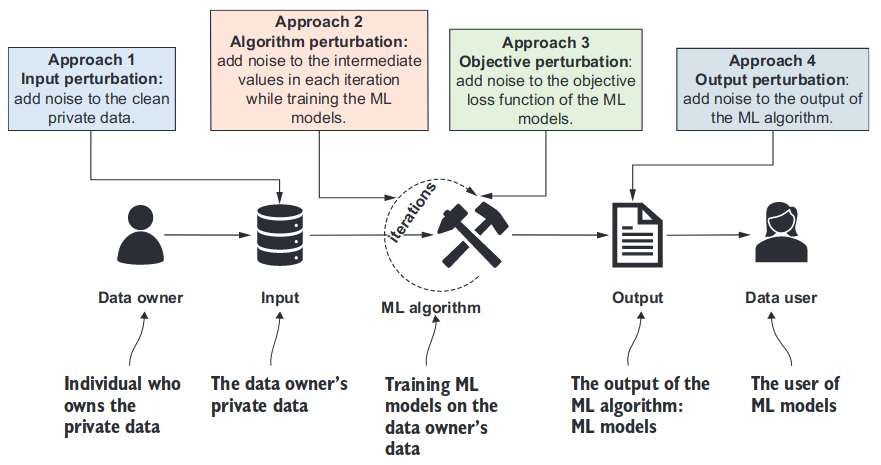
\includegraphics[width=0.7\textwidth]{Graphics/design_principles_dpml.png}
      \caption{Design principles of differentially private ML from \textcite{chang:2023}}
      \label{fig:design_principles_dpml_1}
    \end{figure}
\end{frame}

% evtl noch Algorithmus einfügen?
\begin{frame}{DP in ML}
    \begin{itemize}
        \item<1-> DP-SGD \parencite{abadi:2016} is the \textit{de facto} standard approach
        \begin{itemize}
            \item follows the principle of algorithm pertubation
            \item noise is added to the gradients during training 
        \end{itemize}
        \item<2-> Moments Accountant can provide tighter privacy bounds for this algorithm than classical composition theorems $\rightarrow$ less noise has to be added
        \begin{itemize}
            \item Data must not be processed in fixed size batches, but each data point must be sampled with a certain probability
            \item overall privacy loss can be computed from: 
            \begin{itemize}
                % "klassische" Parameter, die Privacy beeinflussen
                \item \textbf{Noise Scale} and \textbf{Clipping Threshold} % Clipping is done for each example individually, not for the whole batch
                % Parameter die Privacy durch Composition beeinflussen
                \item \textbf{Sampling Rate} and number of steps during training
            \end{itemize}
        \end{itemize}
    \end{itemize}
\end{frame}

\section{Individualized Differential Privacy}

\begin{frame}{Individualized Differential Privacy}
    \begin{itemize}
        \item Users may have different needs regarding their privacy or have different data that doesn't require the same privacy guarantees
        \item DP should fulfill the requirements for each user, not apply overly conservative budgets for the whole dataset \parencite{boenisch:2023}
        \begin{itemize}
            \item $x_i \in \mathcal{G}_p$ with privacy budget $\epsilon_p$
            \item $\mathcal{M}$ satisifies $(\epsilon_p, \delta_p)$-DP if for all datasets $d \sim{} d'$ that only differ in $x_i$ it holds that
            $$\Pr[\mathcal{M}(d) \in S] \leq e^{\epsilon_p} \Pr[\mathcal{M}(d') \in S] + \delta_p$$
        \end{itemize}
    \end{itemize}
\end{frame}

\begin{frame}
    \begin{itemize}
        \item \cite{boenisch:2023} proposed 2 adaptions to DP-SGD
        \begin{enumerate}
            \item \textbf{SCALE}: Individualize Clipping Bounds for different Privacy Groups
            \item \textbf{SAMPLE}: Individualize Sampling Rates for different Privacy Groups
        \end{enumerate}
    \end{itemize}
    \begin{figure}[tb]
        \centering
        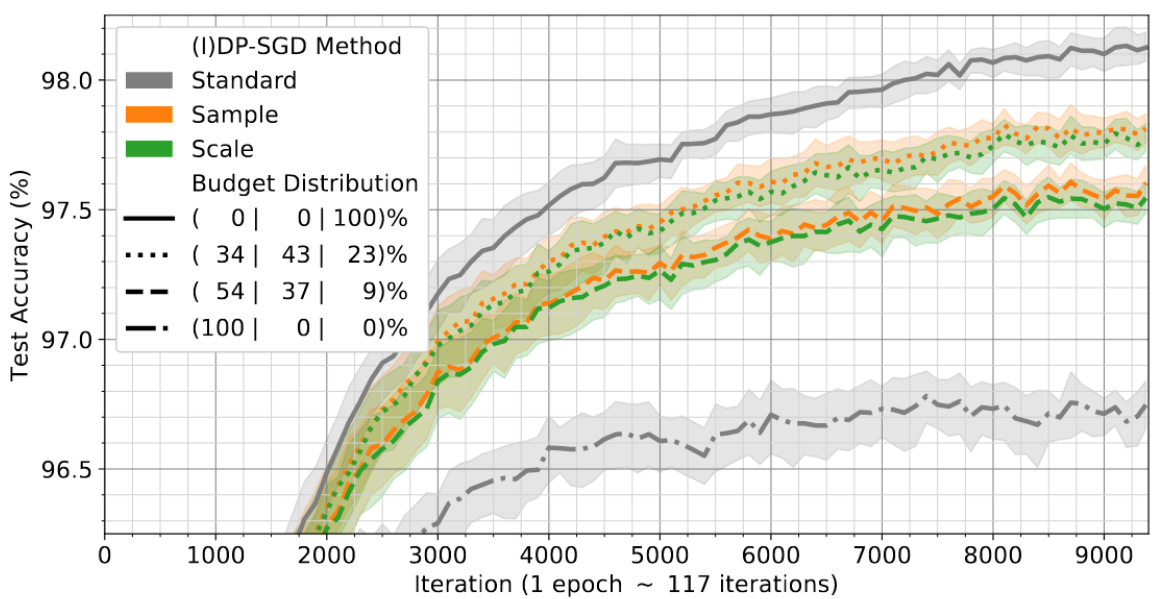
\includegraphics[width=0.6\textwidth]{Graphics/boehnisch_sample_vs_scale.png}
        \label{fig:design_principles_dpml_2}
    \end{figure}
\end{frame}

\begin{frame}{\textbf{SAMPLE}}
    \begin{itemize}
        \item find individual sampling rates $\{q_1, ..., q_P\}$ for the Privacy Groups $\mathcal{G}_i$
        \item find a common Noise Multiplier $\sigma$
        \item keep the original sampling rate $q$ in expectation
        \item idea is to start with the noise multiplier that would be obtained by applying the strictest privacy budget and decrease it iteratively
        % \begin{itemize}
        %     \item in each iteration the sampling rates for each group are recalculated
        % \end{itemize}
        % \item this is done until $q \approx \sum_{p=1}^P \frac{|\mathcal{G}_p|}{N}q_p$
    \end{itemize}
\end{frame}

\section{Federated Learning and DP}

\begin{frame}{Federated Learning}
    \begin{itemize}
        \item various clients, one aggregation server
        \item training is done for $n$ rounds
    \end{itemize}
\end{frame}

\begin{frame}
    \centering
    \begin{tikzpicture}
    
    % Server node
    \node (server) [] {
\includegraphics[width=0.1\textwidth]{Graphics/server.png}};
    
    % % Client nodes
    \node (client1) [below = of server] {
\includegraphics[width=0.1\textwidth]{Graphics/client.png}};
    \node (client2) [right = of client1] {
\includegraphics[width=0.1\textwidth]{Graphics/client.png}};
    \node (client3) [right = of client2] {
\includegraphics[width=0.1\textwidth]{Graphics/client.png}};
    \node (client4) [right = of client3] {
\includegraphics[width=0.1\textwidth]{Graphics/client.png}};
    
    \node<1>[below = 0cm of server] {init parameters};

    \draw<2>[->, >=latex] (server) -- node[midway,right] {send parameters} (client1);
    \draw<2>[->, >=latex] (server) -- (client3);

    \node<3>[below = 0cm of client1] {train locally};
    \node<3>[below = 0cm of client3] {train locally};

    \draw<4>[->, >=latex] (client1) -- node[midway,right] {send updates} (server);
    \draw<4>[->, >=latex] (client3) -- (server);

    \node<5>[right = 0cm of server] {aggregate updates to new parameters};
    
    \end{tikzpicture}
\end{frame}

\begin{frame}{Federated Learning Algorithms}
    \begin{itemize}
        % \item aggregation by calculating a weighted sum 
        % \begin{itemize}
        %     \item weights for a client are proportional to the number of its examples
        % \end{itemize}
        \item \texttt{FedAvg} and \texttt{FedSGD} are simple but widely used FL algorithms
        \begin{itemize}
            \item aggregation is a weighted sum (weights proportional to the size of each client's dataset)
            \item \texttt{FedAvg} allows the clients to train locally for various epochs before sending back the updates
            \item in \texttt{FedSGD} the clients only perform one step locally 
        \end{itemize}
        \item<2-> there are other algorithms, e.g. \texttt{SCAFFOLD} tries to reduce the \textit{client-drift}
    \end{itemize}
\end{frame}

\begin{frame}{Applying DP to FL}
    \begin{itemize}
        \item \textcite{mcmahan:2018} define \textit{user-adjacent} datasets
        \begin{itemize}
            \item $d$, $d'$ are adjacent if $d'$ can be formed by adding or removing all the examples associated with a single user from $d$
        \end{itemize}
        \item<2-> global Differential Privacy
        \begin{itemize}
            \item protects the released model
            \item a trusted third party is needed (the aggregation server)
        \end{itemize}
        \item<3-> local Differential Privacy
        \begin{itemize}
            \item protects client's data against the aggregation server
            \item each client first perturbes its update before sending it to the server
            \item typically leads to a decrease in accuracy
        \end{itemize}
    \end{itemize}
\end{frame}

\begin{frame}{Related Work}
    \begin{itemize}
        \item both \textcite{geyer:2017} and \textcite{mcmahan:2018} came up with similar algorithms
        \begin{itemize}
            \item both focus on protecting the aggregated model (global) and limit the influence on the model of each user
        \end{itemize}
        \item<2-> \textcite{aldaghri:2023} investigate individual Privacy Budgets in the setting of Federated Learning
        \begin{itemize}
            \item they use individual Noise Multipliers similar to the \textbf{SCALE} method of \textcite{boenisch:2023}
            \item also focus on the global setting
            \item their evaluation only considers two groups: "public" and "private" clients
        \end{itemize}
    \end{itemize}
\end{frame}

\begin{frame}{Related Work}
    \begin{itemize}
        \item \textcite{shen:2023}, \textcite{liu:2021}, \textcite{yang:2021} all focus on individual Privacy Budgets in the local setting
        \begin{itemize}
            \item \textcite{shen:2023} define Safe Ranges that can be specified by users
            \item values from those ranges are protected
            \item \textcite{liu:2021} try to identify the most important subspace via singular value decomposition (SVD) among the more public clients and project the more private clients to that space
        \end{itemize}
        \item apart from DP there exist other approaches like secure aggregation for maintaining a better privacy in Federated Learning
    \end{itemize}
\end{frame}

\section{State of my work}

\begin{frame}{State of my Work}
    \begin{itemize}
        \item my approach is based on \texttt{DP-FedAvg} \parencite{mcmahan:2018}
        \begin{itemize}
            \item clients are \textbf{sampled randomly} for each round
            \item local updates are clipped
            \item noise is added on the server (global DP) 
        \end{itemize}
        \item<2-> sampling rates and noise multiplier are calculated based on \textbf{SAMPLE} from \textcite{boenisch:2023} using the definition of \textit{user-adjacent} datasets
        \begin{itemize}
            \item calculate Noise Multiplier and sampling rates with their algorithm
            \item then plug those into \texttt{DP-FedAvg}
        \end{itemize}
    \end{itemize}
\end{frame}

\begin{frame}{Experiments}
\begin{table}[]
    \centering
    \begin{tabular}{|c|c|c|c|c|}
        \hline
        $\epsilon$ & strict & individual-strict & individual-relaxed & relaxed \\
        \hline
        1.0 & 100\% & 54\% & 34\% & - \\
        2.0 & - & 37\% & 43\% & - \\
        3.0 & - & 9\% & 23\% & 100\% \\
        \hline
    \end{tabular}
    \label{tab:experiment-setup}
\end{table}
    \begin{itemize}
        \item so far only evaluated on MNIST dataset from Tensorflow Federated (TFF) (non-i.i.d.)
        \item all experiments were run for 100 rounds, 100 clients per round and $\delta = 10^{-5}$
        \item the model is a simple multilayer dense neural network
    \end{itemize}
\end{frame}

\begin{frame}{Results}
    \begin{columns}
        \begin{column}{0.5\textwidth}
            \begin{figure}[tb]
                \centering
                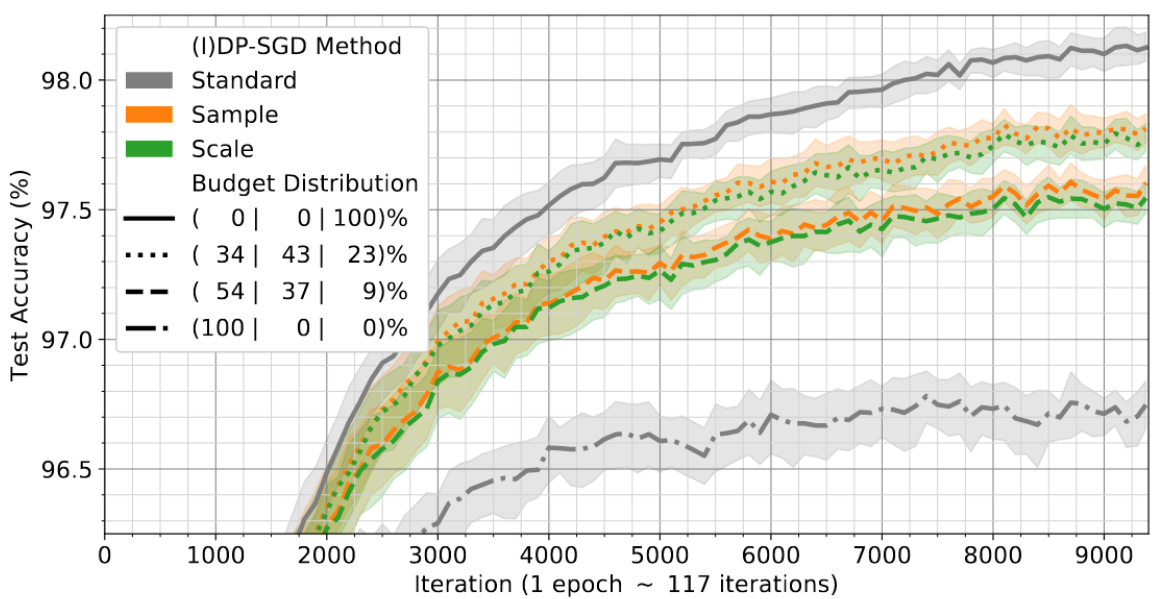
\includegraphics[width=\textwidth]{Graphics/boehnisch_sample_vs_scale.png}
                \label{fig:design_principles_dpml}
            \end{figure}
        \end{column}
        \begin{column}{0.5\textwidth}
            \begin{figure}
                \centering
                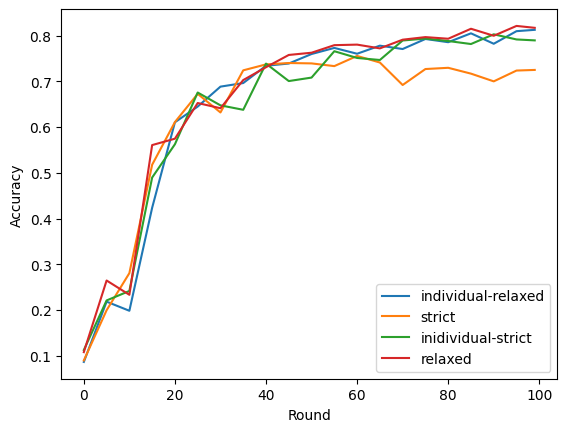
\includegraphics[width=\textwidth]{Graphics/accuracy.png}
                \label{fig:enter-label}
            \end{figure}
        \end{column}
    \end{columns}
\end{frame}

\subsection{Outlook}

\begin{frame}{Next up}
    \begin{itemize}
        \item train completely without DP to see which results are possible
        \begin{itemize}
            \item also in relation to non-federated SOTA results
        \end{itemize}
        \item \textcite{boenisch:2023} use \texttt{MNIST}, \texttt{SVHN} and \texttt{CIFAR10} datasets
        \begin{itemize}
            \item for comparison I want to integrate those into TFF (i.i.d.)
        \end{itemize}
        \item use a better suited neural network
        \begin{itemize}
            \item so far my investigations centered on DP and adjustments to the algorithms
            \item but this will be important to compare my work to others
        \end{itemize}
    \end{itemize}
\end{frame}

\begin{frame}{Sensitivity of my Algorithm}
    \begin{itemize}
        \item the updates of each individual client are bounded
        \item the aggregation of those updates has to have a bounded sensitivity
        \item \textcite{mcmahan:2018} define two aggregations with bounded sensitivity and end up using $\tilde{f}_f$ 
        $$\tilde{f}_f(\mathcal{C}) = \frac{\sum_{k \in \mathcal{C}} w_k \Delta_k}{qW}\text{, where } W = \sum_{j} w_j$$
        \item $\tilde{f}_f$ has a bounded sensitivity of $S(\tilde{f}_f) \leq \frac{S}{qW}$
    \end{itemize}
\end{frame}

\begin{frame}{Sensitivity of my Algorithm}
    \begin{itemize}
        \item Using $\tilde{f}_f$ from \texttt{DP-FedAvg} the sensitivity should still be bounded
        \begin{itemize}
            \item but $qW = q \sum_{k}w_k$ isn't an unbiased estimator anymore when using individual $q_k$'s
            \item my plan is to "adjust" the computation to $\sum_k q_k w_k$
        \end{itemize}
        \item in practice Adaptive Clipping \parencite{andrew:2021} is used to set the Clipping Bounds on the client side in each round
        \begin{itemize}
            \item in my opinion that should still work using my approach
        \end{itemize}
    \end{itemize}
\end{frame}

% \begin{frame}{Next Up}
% % Noch einmal erwähnen, dass ich vorhabe mir die Definition meiner DP noch einmal vorzunehmen (IDP + User adjacent)
%     \begin{itemize}
%         \item 
%     \end{itemize}
% \end{frame}

\begin{frame}{Open Questions}
    \begin{itemize}
        \item Is my approach valid and how could I profe that (empirically)?
        \begin{itemize}
            \item Formal proofs?
            \item Privacy attacks?
        \end{itemize}
        % \begin{itemize}
        %     \item is it valid to use the tools provided by \textcite{boenisch:2023} and use them in the new environment of clients instead of data points?
        %     \item is it okay to transfer the notion of privacy from datapoints to Clients
        %     \item imo the most critical point is the calculation of the Sensitivity
        % \end{itemize}
        % \item How to treat the individuals' privacy preferences? Is it valid for the server to have access to them without DP-Mechanisms?
    \end{itemize}
\end{frame}

\section{Summary}

\begin{frame}{Summary}
    \begin{itemize}
        \item my goal is to combine individual DP with FL
        \item as far as I know there hasn't been an attempt to do that using individual sampling rates
        \item to individualize DP using individual sampling rates seems promising based on the results of \textcite{boenisch:2023}
        \item I want to verify its effectiveness by evaluating my approach against others on public benchmark datasets
    \end{itemize}    
\end{frame}
  
% \begin{frame}{My topic is important\dots }
% \begin{itemize}
%   \item Here is some general statement 
%   \item More information about my topic includes these points: 
%     \begin{itemize}
%       \item A thought
%       \item Another idea
%       \item A related thing 
%       \item \dots
%     \end{itemize}
% \end{itemize}
% \end{frame}


% \begin{frame}{\dots but it is a difficult task}
%   Because of reasons
%   \begin{block}{Block title}
%     I am a block environment 
%   \end{block}
% \end{frame}


% \section[A short section title]{I am a longer section title}

% \begin{frame}

% \end{frame}


% \section{Summary}


% \begin{frame}

% \end{frame}

% \begin{frame}

% \end{frame}

% \begin{frame}

% \end{frame}

% \begin{frame}

% \end{frame}

% \begin{frame}

% \end{frame}

\begin{frame}[allowframebreaks]{Bibliography}
\printbibliography
\end{frame}

\end{document}
